\documentclass{bioinfo}
\copyrightyear{2017} \pubyear{2017}

\usepackage{amsmath}
\usepackage{listings}
\usepackage{algorithm}
\usepackage{algorithmic}
\usepackage{amsthm}
\usepackage{graphicx}
\usepackage{url}

\newtheorem{defn}{Definition}
\newtheorem{lemma}{Lemma}

\access{Advance Access Publication Date: Day Month Year}
\appnotes{Manuscript Category}

\begin{document}
\firstpage{1}

\subtitle{Subject Section}

\title[Distributed Variant Calling with Avocado]{Distributed Variant Calling with Avocado}
\author[Nothaft \textit{et~al}.]{Frank~Austin~Nothaft\,$^{\text{\sfb 1,2}*}$, David~A.~Patterson\,$^{\text{\sfb 1,2}}$ and Anthony~D.~Joseph\,$^{\text{\sfb 1}}$}
\address{$^{\text{\sf 1}}$AMPLab, University of California, Berkeley, 94720, USA and \\
$^{\text{\sf 2}}$ASPIRE Lab, University of California, Berkeley, 94720, USA.}

\corresp{$^\ast$To whom correspondence should be addressed.}

\history{Received on XXXXX; revised on XXXXX; accepted on XXXXX}

\editor{Associate Editor: XXXXXXX}

\abstract{\textbf{Motivation:} With the increasing size of genomic datasets, computational
analysis is a rate limiting step. Variant calling is a particularly expensive step, especially
when working with whole genome data. To improve performance, we implement variant calling on
top of the horizontally scalable Apache Spark distributed computing framework. \\
\textbf{Results:} Avocado achieves linear scalability with the size of the computing cluster,
while achieving state-of-the-art accuracy in SNP calling, and competitive accuracy at INDEL
calling. \\
\textbf{Availability:} Avocado is open source software, released under the
Apache 2 license. The Avocado source code is hosted at
\href{https://github.com/bigdatagenomics/avocado}{https://github.com/bigdatagenomics/avocado}. \\
\textbf{Contact:} \href{fnothaft@berkeley.edu}{fnothaft@berkeley.edu}}

\maketitle

\section{Introduction}

While many modern short-read based variant callers can achieve greater than
99\% accuracy when calling single nucleotide variants~(SNVs), accuracy decreases
when calling insertion/deletion~(INDEL) variants. For INDELs that are shorter
than the read length, some degradation in accuracy is caused by incorrect
mapping of reads containing INDELs. However, this is not the primary culprit.
While most reads map correctly, they
are frequently locally misaligned. In short, these reads have been placed in
the correct area of the reference genome, but their local alignment makes them
appear to represent a different sequence variant then they truly contain.

There are two general approaches that can be used to eliminate the effect of
incorrect local alignment on variant calling accuracy: we can either use a local
sequence alignment algorithm that is less likely to misrepresent INDEL variants
when aligning individual reads, or we can try to improve the alignments of all
reads that have mapped around a genomic locus by pooling and jointly realigning
these reads. Most tools have focused on the second approach, which further
bifurcates into realignment-only and reassembly-with-realignment algorithms.
Research has focused on realignment-based approaches because realignment-based
approaches obliviate the major problem with traditional local sequence alignment
algorithms~\citep{smith81, ukkonen85, landau86}, which by their probabilistic or
dynamic nature cannot be guaranteed to emit consistent alignments for all reads
that contain an INDEL variant. Realignment algorithms eliminate
this problem by identifying all possible INDELs in the reads at the site,
scoring these variants at the site, and realigning the reads to contain a
consistent representation of the top scoring variant(s).

Although realignment and reassembly algorithms have high accuracy, they also
have high computational cost. The traditional formulation of a realignment
algorithm has $\mathcal{O}(n^4)$ runtime complexity, while most local sequence
alignment algorithms have runtime complexity of $\mathcal{O}(n^2)$ or lower.
Additionally, realignment approaches require all of the reads covering a
genomic locus to be materialized which necessitates a shuffle of the input
dataset and can have significant memory requirements. While the end-to-end
runtime can be decreased by only reassembling a portion of the genome, the
performance improvements available through these approaches are bound similarly
to Amdahl's law: local assembly is sufficiently expensive that an approach that
prefilters 90\% of the genome only achieves a $3\times$ improvement in
end-to-end runtime~\citep{bloniarz14}.

As an alternative to traditional realignment and reassembly approaches, we
introduce a local sequence alignment algorithm that is inspired by colored de
Bruijn graphs~\citep{iqbal12}. This algorithm has several desirable properties:
it has linear runtime complexity and it produces provably canonical pairwise
alignments. When used for locally realigning previously mapped reads, we can
determine if an individual read is already canonically aligned prior to
realigning, which allows us to aggressively limit the number of reads realigned.
Our algorithm uses motifs that we have identified in the structure of the
sequence flanking a bubble in a colored de Bruijn graph. Our algorithm has an
efficient implementation and we can prove strong guarantees about the local
alignments that our algorithm generates. We have implemented this algorithm in
\textsc{Avocado}, a parallel variant caller implemented using \textsc{Apache
Spark}~\citep{zaharia12, zaharia10} and the \textsc{ADAM} library for parallel
genomic analysis~\citep{massie13, nothaft15}. Our approach achieves a $10\times$
speedup over conventional INDEL realignment tools when run on a single node
while maintaining variant calling accuracy, and can be parallelized across a
cluster of computers. Our implementation is released as open source code under
an Apache 2 license and is available from
\url{https://github.com/bigdatagenomics/avocado}.

\section{Approach}

The accuracy of insertion and deletion~(INDEL) variant discovery has been improved by the development
of variant callers that couple local reassembly with haplotype-based statistical models to recover INDELs
that were locally misaligned~\citep{albers11}. Now, several prominent variant callers such as the Genome
Analysis Toolkit's~(GATK) \textsc{HaplotypeCaller}~\citep{depristo11}, \textsc{Scalpel}~\citep{narzisi14}, and
\textsc{Platypus}~\citep{rimmer14}. Although haplotype-based methods have enabled more accurate INDEL
and single nucleotide polymorphism~(SNP) calls~\citep{bao14}, this accuracy comes at the cost of
end-to-end runtime~\citep{talwalkar14}. Several recent projects have been focused on improving
reassembly cost either by limiting the percentage of the genome that is reassembled~\citep{bloniarz14} or
by improving the performance of algorithms of the core algorithms used in local
reassembly~\citep{rimmer14}.

The performance issues seen in haplotype reassembly approaches derives from the high asymptotic
complexity of reassembly algorithms. Although specific implementations may vary slightly, a typical
local reassembler performs the following steps:

\begin{enumerate}
\item A de Bruijn graph is constructed from the reads aligned to a region of the reference genome,
\item All valid paths~(\emph{haplotypes}) between the start and end of the graph are enumerated,
\item Each read is realigned to each haplotype, typically using a pair Hidden Markov Model~(HMM,
see~\citet{durbin98}),
\item A statistical model uses the read$\leftrightarrow$haplotype alignments to choose the haplotype pair
that most likely represents the variants hypothesized to exist in the region, 
\item The alignments of the reads to the chosen haplotype pair are used to generate statistics that are
then used for genotyping.
\end{enumerate}

In this paper, we focus on steps one through three of the local reassembly problem, as there is wide
variation in the algorithms used in stages four and five. Stage one (graph
creation) has approximately $\mathcal{O}(r l_r)$ time complexity, and stage two (graph elaboration) has
$\mathcal{O}(h \max(l_h))$ time complexity.
The asymptotic time cost bound of local reassembly comes from stage three, where cost is $\mathcal{O}(h r l_r
\max(l_h))$, where $h$ is the number of haplotypes tested in this region\footnote{The number of
haplotypes tested may be lower than the number of haplotypes reassembled. Several tools
(see~\citet{depristo11, garrison12}) allow users to limit the number of haplotypes evaluated to improve
performance.}, $r$ is the number of reads aligned to this region, $l_r$ is the read length\footnote{For
simplicity, we assume constant read length. This is a reasonable assumption as many of the variant
callers discussed target Illumina reads that have constant length.}, and $\min(l_h)$ is the length of the
shortest haplotype that we are evaluating. This complexity comes from realigning $r$ reads to $h$
haplotypes, where realignment has complexity $\mathcal{O}(l_r l_h)$.

In this paper, we introduce the indexed de Bruijn graph and demonstrate how it can be used to
reduce the asymptotic complexity of reassembly. An indexed de Bruijn graph is identical to a
traditional de Bruijn graph, with one modification: when we create the graph, we annotate each
$k$-mer with the index position of that $k$-mer in the sequence it was observed in. This simple addition
enables the use of the indexed de Bruijn graph for $\Omega(n)$ local sequence alignment with
canonical edit representations for most edits. This structure can be used for both sequence alignment and
assembly, and achieves a more efficient approach for variant discovery via local reassembly.

Current variant calling pipelines depend heavily on realignment based approaches for accurate
genotyping~\citep{li14}. Although there are several approaches that do not make explicit use of reassembly,
all realignment based variant callers use an algorithmic structure similar to the one described
above. In non-assembly approaches like \textsc{FreeBayes}~\citep{garrison12}, stages
one and two are replaced with a single step where the variants observed in the reads aligned to a given
haplotyping region are filtered for quality and integrated directly into the reference haplotype in that region.
In both approaches, local alignment errors~(errors in alignment \emph{within} this region) are corrected
by using a statistical model to identify the most likely location that the read could have come from, given
the other reads seen in this area.

Although the model used for choosing the best haplotype pair to finalize realignments to varies between
methods~(e.g., the GATK's \textsc{IndelRealigner} uses a simple log-odds model~\citep{depristo11}, while
methods like \textsc{FreeBayes}~\citep{garrison12} and \textsc{Platypus}~\citep{rimmer14} make use of richer
Bayesian models), these methods require an all-pairs alignment of reads to candidate
haplotypes. This leads to the runtime complexity bound of $\mathcal{O}(h r l_r \min(l_h))$
, as we must realign $r$ reads to $h$ haplotypes, where the cost of realigning
one read to one haplotype is $\mathcal{O}(l_r \max(l_h))$, where $l_r$ is the read length~(assumed to be
constant for Illumina sequencing data) and $\max(l_h)$ is the length of the longest haplotype. Typically,
the data structures used for realignment~($\mathcal{O}(l_r \max(l_h))$ storage cost) can be reused.
These methods typically retain \emph{only} the best local realignment per read per haplotype, thus
bounding storage cost at $\mathcal{O}(h r)$.

For non-reassembly based approaches, the cost of generating candidate haplotypes is $\mathcal{O}(r)$,
as each read must be scanned for variants, using the pre-existing alignment. These variants are typically
extracted from the CIGAR string, but may need to be normalized~\citep{li14}. de Bruijn graph based 
reassembly methods have similar $\mathcal{O}(r)$ time complexity for building the de Bruijn
graph as each read must be sequentially broken into $k$-mers, but these methods have a different
storage cost. Specifically, storage cost for a de Bruijn graph is similar to $\mathcal{O}(k
(l_{\text{ref}} + l_{\text{variants}} + l_{\text{errors}}))$, where $l_{\text{ref}}$ is the length of the reference
haplotype in this region, $l_{\text{variants}}$ is the length of true variant sequence in this region, 
$l_{\text{errors}}$ is the length of erroneous sequence in this region, and $k$ is the $k$-mer size. In
practice, we can approximate both errors and variants as being random, which gives $\mathcal{O}(k
l_{\text{ref}})$ storage complexity. From this graph, we must enumerate the haplotypes present in the
graph. Starting from the first $k$-mer in the reference sequence for this region, we perform a depth-first
search to identify all paths to the last $k$-mer in the reference sequence. Assuming that the graph is
acyclic~(a common restriction for local assembly), we can
bound the best case cost of this search at $\Omega(h \min l_h)$.

The number of haplotypes evaluated, $h$, is an important contributor to the algorithmic complexity of
reassembly pipelines, as it sets the storage and time complexity of the realignment scoring phase, the
time complexity of the haplotype enumeration phase, and is related to the storage complexity of the
de Bruijn graph. The best study of the complexity of assembly techniques was done by Kingsford
et al.~\citep{kingsford10}, but is focused on \emph{de novo} assembly and pays special attention to
resolving repeat structure. In the local realignment case, the number of haplotypes identified is determined
by the number of putative variants seen. We can na\"{i}vely model this cost with \eqref{eq:haplotypes},
where $f_v$ is the frequency with which variants occur, $\epsilon$ is the rate at which bases are
sequenced erroneously, and $c$ is the coverage (read depth) of the region.

\begin{align}
\label{eq:haplotypes}
h \sim f_v l_{\text{ref}} + \epsilon l_{\text{ref}} c
\end{align}

This model is na\"{i}ve, as the coverage depth and rate of variation varies across sequenced datasets,
especially for targeted sequencing runs~\citep{fang14}. Additionally, while the $\epsilon$ term models the
total number of sequence errors, this is not completely correlated with the number of \emph{unique}
sequencing errors, as sequencing errors are correlated with sequence context~\citep{depristo11}. Many
current tools allow users to limit the total number of evaluated haplotypes, or apply strategies to minimize
the number of haplotypes considered, such as filtering observed variants that are likely to be sequencing
errors~\citep{garrison12}, restricting realignment to INDELs~(\textsc{IndelRealigner},~\citep{depristo11}), or
by trimming paths from the assembly graph. Additionally, in an de Bruijn graph, errors in the
first $k$ or last $k$ bases of a read will manifest as spurs and will not contribute paths through the graph. We provide~\eqref{eq:haplotypes} solely as a motivating
approximation, and hope to study these characteristics in more detail in future work.

\begin{methods}
\section{Methods}

To use Avocado to call variants, we run two applications, each of which has several
sub-stages:

\begin{enumerate}
\item \textbf{INDEL Reassembly:} Here, we clean up all reads that are aligned
near INDEL variants. We do this as a two step process:
\begin{enumerate}
\item We make a pass over all reads, using our ``bubble flank motif'' algorithm
to extract INDEL variants. These INDEL variants are collected on a single node,
and used as inputs to the next stage.
\item We run \textsc{ADAM}'s~\citep{massie13, nothaft15} INDEL realigner, using the
discovered INDELs from stage one as ``known INDELs'' to realign to.
\end{enumerate}
\item \textbf{Variant Calling:} In this phase, we discover all SNVs and INDELs,
score them using the reads, and emit either called variants or genotype
likelihoods in genome VCF~(gVCF) format. This runs as a four step process:
\begin{enumerate}
\item We extract all variants from the aligned reads by parsing the alignments.
\item Using these variants, we compute all read/variant overlaps, and compute
the likelihood that each read represents a given variant that it overlaps. In
gVCF mode, we also calculate the likelihood of the reference allele at all
locations covered by a read.
\item We merge all of the per-read likelihoods per variant. This gives us final
genotype likelihoods per each variant.
\item Finally, we apply a standard set of hard filters to each variant.
\end{enumerate}
\end{enumerate}

All of these stages are implemented as a parallel application that runs on top of
\textsc{Apache Spark}~\citep{zaharia10, zaharia12}, using the \textsc{ADAM}
library~\citep{massie13, nothaft15}.

\subsection{INDEL Reassembly}
\label{sec:indel-reassembly}

As opposed to traditional realignment based approaches, we canonicalize INDELs
in the reads by looking for ``bubble flank motifs.'' In a colored de Bruijn
graph, a bubble refers to a location where the graph diverges between two
samples. In \S\ref{sec:formulation}, we demonstrate how we can use the
reconvergence of the de Bruijn graph in the flanking sequence around a bubble
to define provably canonical alignments of the bubble between two sequences.
For a colored de Bruijn graph containing reads and the reference genome, this
allows us to canonically express INDEL variants in the reads against the
reference. In \S\ref{sec:implementation}, we then show how this approach
can be implemented efficiently without building a de Bruijn graph per read,
or even adding each read to a de Bruijn graph. Once we have extracted a
canonical set of INDELs, we realign the reads to each INDEL sequence using
\textsc{ADAM}'s INDEL realigner, in known INDELs mode. For a full description
of the INDEL realignment process, see~\citet{nothaft15avocado}.

\subsubsection{Preliminaries}
\label{sec:formulation}

Our method relies on an \emph{indexed de Bruijn} graph, which is a slight
extension of the colored de Bruijn graph~\citep{iqbal12}. Specifically, each
$k$-mer in an indexed de Bruijn graph knows which sequence position~(index)
it came from in it's underlying read/sequence. To construct an indexed de
Bruijn graph, we start with the traditional formulation of a \emph{de Brujin}
graph for sequence assembly:

\begin{defn}[de Bruijn Graph]
\label{defn:dbg}
A de Bruijn graph describes the observed transitions between adjacent $k$-mers in a sequence. Each
$k$-mer $s$ represents a $k$-length string, with a $k - 1$ length prefix given by $\text{prefix}(s)$ and a
length 1 suffix given by $\text{suffix}(s)$. We place a directed edge ($\rightarrow$) from $k$-mer $s_1$ to
$k$-mer $s_2$ if $\text{prefix}(s_1)^{\{1, k - 2\}} + \text{suffix}(s_1) = \text{prefix}(s_2)$.
\end{defn}

Now, suppose we have $n$ sequences $\mathcal{S}_1, \dots, \mathcal{S}_n$. Let us assert that for each
$k$-mer $s \in \mathcal{S}_i$, then the output of function $\text{index}_i(s)$ is defined. This function
provides us with the integer position of $s$ in sequence $\mathcal{S}_i$. Further, given two $k$-mers
$s_1, s_2 \in \mathcal{S}_i$, we can define a distance function
$\text{distance}_i(s_1, s_2) = | \text{index}_i(s_1) - \text{index}_i(s_2) |$. To create an indexed
de Bruijn graph, we simply annotate each $k$-mer $s$ with the $\text{index}_i(s)$ value for all
$\mathcal{S}_i, i \in \{1, \dots, n\}$ where $s \in \mathcal{S}_i$. This index value is trivial to log when
creating the original de Bruijn graph from the provided sequences.

Let us require that all sequences $\mathcal{S}_1, \dots, \mathcal{S}_n$ are not repetitive, which implies
that the resulting de Bruijn graph is acyclic. If we select any two sequences $\mathcal{S}_i$ and
$\mathcal{S}_j$ from $\mathcal{S}_1, \dots, \mathcal{S}_n$ that share at least two $k$-mers $s_1$ and
$s_2$ with common ordering~($s_1 \rightarrow \dots \rightarrow s_2$ in both $\mathcal{S}_i$ and
$\mathcal{S}_j$), the indexed de Bruijn graph $G$ provides several guarantees:

\begin{enumerate}
\item If two sequences $\mathcal{S}_i$ and $\mathcal{S}_j$ share at least two $k$-mers $s_1$ and
$s_2$, we can provably find the maximum edit distance $d$ of the subsequences in $\mathcal{S}_i$ and
$\mathcal{S}_j$, and bound the cost of finding this edit distance at $\mathcal{O}(nd)$,\footnote{Here,
$n = \max(\text{distance}_{\mathcal{S}_i}(s_1, s_2), \text{distance}_{\mathcal{S}_j}(s_1, s_2))$.}
\item For many of the above subsequence pairs, we can bound the cost at $\mathcal{O}(n)$, \emph{and}
provide canonical representations for the necessary edits,
\item $\mathcal{O}(n^2)$ complexity is restricted to aligning the subsequences of $\mathcal{S}_i$ and
$\mathcal{S}_j$ that exist \emph{before} $s_1$ or \emph{after} $s_2$.
\end{enumerate}

Let us focus on cases 1 and 2, where we are looking at the subsequences of $\mathcal{S}_i$ and
$\mathcal{S}_j$ that are between $s_1$ and $s_2$. A trivial case arises when both $\mathcal{S}_i$ and
$\mathcal{S}_j$ contain an identical path between $s_1$ and $s_2$ (i.e.,
$s_1 \rightarrow s_n \rightarrow \dots \rightarrow s_{n + m} \rightarrow s_2$ and
$s_{n + k} \in \mathcal{S}_i \wedge s_{n + k} \in \mathcal{S}_j \forall k \in \{0, \dots , m\}$). Here, the
subsequences are clearly identical. This determination can be made trivially by walking from vertex $s_1$
to vertex $s_2$ with $\mathcal{O}(m)$ cost.

However, three distinct cases can arise whenever $\mathcal{S}_i$ and $\mathcal{S}_j$ diverge between
$s_1$ and $s_2$. For simplicity, let us assume that both paths are independent~(see
Definition~\ref{defn:path-independence}). These three cases correspond to there being either a canonical
substitution edit, a canonical INDEL edit, or a non-canonical (but known distance) edit between
$\mathcal{S}_i$ and $\mathcal{S}_j$.

\begin{defn}[Path Independence]
\label{defn:path-independence}
Given a non-repetitive de Bruijn graph $G$ constructed from $\mathcal{S}_i$ and $\mathcal{S}_j$, we say
that $G$ contains independent paths between $s_1$ and $s_2$ if we can construct two subsets
$\mathcal{S}'_i \subset \mathcal{S}_i, \mathcal{S}'_j \subset \mathcal{S}_j$ of $k$-mers where $s_{i + n}
\in \mathcal{S}'_i \forall n \in \{0, \dots, m_i\}, s_{i + n - 1} \rightarrow s_{i + n} \forall n \in \{1, \dots, m_i\}$,
$s_{j + n} \in \mathcal{S}'_j \forall n \in \{0, \dots, m_j\}, s_{j + n - 1} \rightarrow s_{j + n} \forall n \in \{1,
\dots, m_j\}$, and $s_1 \rightarrow s_i, s_j; s_{i + m_i}, s_{j + m_j} \rightarrow s_2$ and $\mathcal{S}'_i
\bigcap \mathcal{S}'_j = \emptyset$, where $m_i = \text{distance}_{\mathcal{S}_i}(s_1, s_2)$, and $m_j =
\text{distance}_{\mathcal{S}_j}(s_1, s_2)$. This implies that the sequences $\mathcal{S}_i$ and
$\mathcal{S}_j$ are different between $s_1, s_2$,
\end{defn}

We have a canonical substitution edit if $m_i = m_j = k$, where $k$ is the $k$-mer size. Here, we can
prove that the edit between $\mathcal{S}_i$ and $\mathcal{S}_j$ between $s_1, s_2$ is a single base
substitution $k$ letters after $\text{index}(s_1)$:

\begin{proof}[Proof regarding Canonical Substitution]
\label{proof:canonical-substitution}
Suppose we have two non-repetitive sequences, $\mathcal{S}_i'$ and $\mathcal{S}_j'$, each of length
$2k + 1$. Let us construct a de Bruijn graph $G$, with $k$-mer length $k$. If each sequence begins with
$k$-mer $s_1$ and ends with $k$-mer $s_2$, then that implies that the first and last $k$ letters of
$\mathcal{S}_i'$ and $\mathcal{S}_j'$ are identical. If both subsequences had the same character at
position $k$, this would imply that both sequences were identical and therefore the two paths between
$s_1, s_2$ would not be independent~(Definition~\ref{defn:path-independence}). If the two letters are
different \emph{and} the subsequences are non-repetitive, each character is responsible for $k$
previously unseen $k$-mers. This is the only possible explanation for the two independent $k$ length
paths between $s_1$ and $s_2$.
\end{proof}

To visualize the graph corresponding to a substitution, take the two example sequences \texttt{CCACTGT}
and \texttt{CCAATGT}. These two sequences differ by a \texttt{C} $\leftrightarrow$ \texttt{A} edit at
position three. With $k$-mer length $k = 3$, this corresponds to the graph in Figure~\ref{fig:sne}.

\begin{figure}[h]
\begin{center}
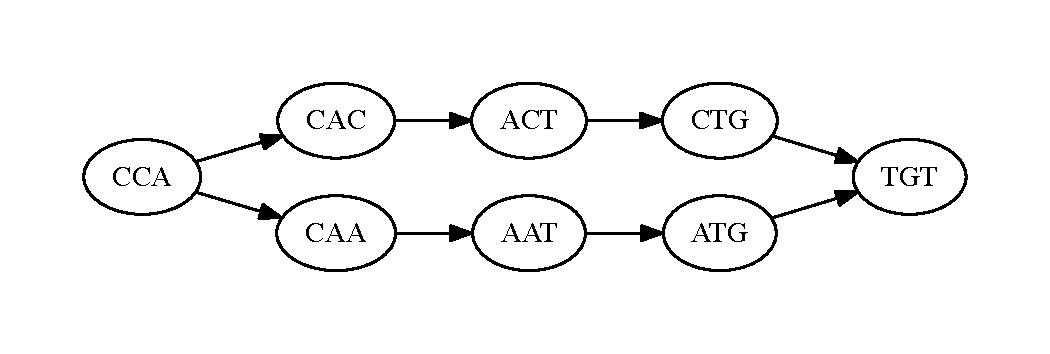
\includegraphics[width=0.95\linewidth, clip=true, trim=0 39 0 39]{graphs/sne.pdf}
\end{center}
\caption{Subgraph Corresponding To a Single Nucleotide Edit}
\label{fig:sne}
\end{figure}

If $m_i = k - 1, m_j \ge k$ or vice versa, we have a canonical INDEL edit (for convenience, we assume
that $\mathcal{S}_i'$ contains the $k - 1$ length path). Here, we can prove that there is a $m_j - m_i$
length insertion\footnote{This is equivalently a $m_j - m_i$ length deletion in $\mathcal{S}_i'$ relative to
$\mathcal{S}_j'$.} in $\mathcal{S}_j'$ relative to $\mathcal{S}_i'$, $k - 1$ letters \emph{after}
$\text{index}(s_1)$:

\begin{lemma}[Distance between $k$ length subsequences]
\label{lem:minimum-distance}
\emph{Indexed de Bruijn} graphs naturally provide a distance metric for $k$ length substrings. Let us construct an
indexed de Bruijn graph $G$ with $k$-mers of length $k$ from a non-repetitive sequence $\mathcal{S}$.
For any two $k$-mers $s_a, s_b \in \mathcal{S}, s_a \ne s_b$, the
$\text{distance}_\mathcal{S}(s_a, s_b)$ metric is equal to $l_p + 1$, where $l_p$ is the length of the
path (in $k$-mers) between $s_a$ and $s_b$. Thus, $k$-mers with overlap of $k - 1$ have an edge
directly between each other ($l_p = 0$) and a distance metric of 1. Conversely, two $k$-mers that are
adjacent but not overlapping in $\mathcal{S}$ have a distance metric of $k$, which implies $l_p = k - 1$.
\end{lemma}

\begin{proof}[Proof regarding Canonical INDELs]
\label{proof:canonical-indels}
We are given a graph $G$ which is constructed from two non-repetitive sequences $\mathcal{S}_i'$ and
$\mathcal{S}_j'$, where the only two $k$-mers in both $\mathcal{S}_i'$ and $\mathcal{S}_j'$ are $s_1$
and $s_2$ and both sequences provide independent paths between $s_1$ and $s_2$. By
Lemma~\ref{lem:minimum-distance}, if the path from $s_1 \rightarrow \dots \rightarrow s_2 \in
\mathcal{S}_i'$ has length $k - 1$, then $\mathcal{S}_i'$ is a string of length $2k$ that is formed by
concatenating $s_1, s_2$. Now, let us suppose that the path from $s_1 \rightarrow \dots \rightarrow s_2
\in \mathcal{S}_j'$ has length $k + l - 1$. The first $l$ $k$-mers after $s_1$ will introduce a $l$ length
subsequence $\mathcal{L} \subset \mathcal{S}_j', \mathcal{L} \not\subset \mathcal{S}_i'$, and then the
remaining $k - 1$ $k$-mers in the path provide a transition from $\mathcal{L}$ to $s_2$. Therefore,
$\mathcal{S}_j'$ has length of $2k + l$, and is constructed by concatenating $s_1, \mathcal{L}, s_2$.
This provides a canonical placement for the inserted sequence $\mathcal{L}$ in $\mathcal{S}_j'$ between
$s_1$ and $s_2$.
\end{proof}

To visualize the graph corresponding to a canonical INDEL, take the two example sequences
\texttt{CACTGT} and \texttt{CACCATGT}. Here, we have a \texttt{CA} insertion after position two. With
$k$-mer length $k = 3$, this corresponds to the graph in Figure~\ref{fig:indel}.

\begin{figure}[h]
\begin{center}
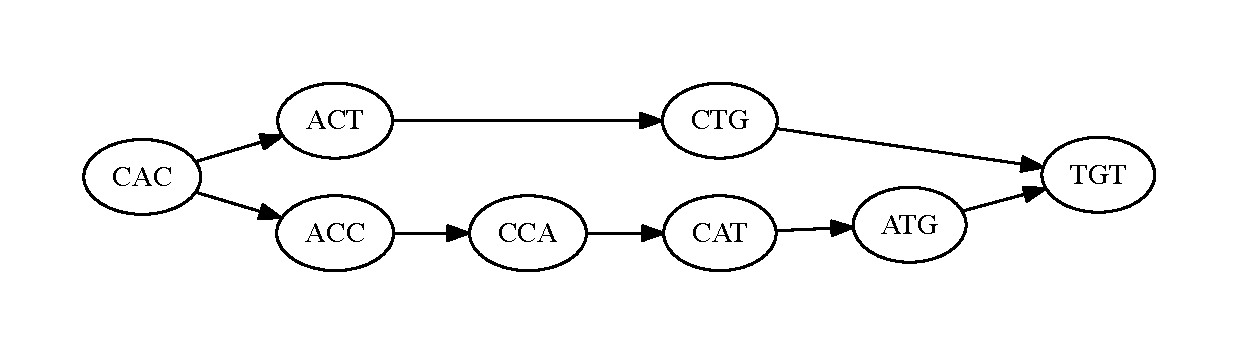
\includegraphics[width=0.95\linewidth, clip=true, trim=0 39 0 39]{graphs/indel.pdf}
\end{center}
\caption{Subgraph Corresponding To a Canonical INDEL Edit}
\label{fig:indel}
\end{figure}

Where we have a canonical allele, the cost of computing the edit is set by the need to walk the graph
linearly from $s_1$ to $s_2$, and is therefore $\mathcal{O}(n)$. However, in practice, we will see
differences that cannot be described as one of the earlier two canonical approaches. First, let us
generalize from the two above proofs: if we have two independent paths between $s_1, s_2$ in the
de Bruijn graph $G$ that was constructed from $\mathcal{S}_i, \mathcal{S}_j$, we can describe
$\mathcal{S}_i$ as a sequence created by concatenating $s_1, \mathcal{L}_i, s_2$.\footnote{This
property holds true for $\mathcal{S}_j$ as well.} The canonical edits merely result from special cases:

\begin{itemize}
\item In a canonical substitution edit, $l_{\mathcal{L}_i} = l_{\mathcal{L}_j} = 1$.
\item In a canonical INDEL edit, $l_{\mathcal{L}_i} = 0, l_{\mathcal{L}_j} \ge 1$.
\end{itemize}

Conceptually, a non-canonical edit occurs when two edits occur within $k$ positions of each other. In
this case, we can trivially fall back on a $O(nm)$ local alignment algorithm~(e.g., a pairwise HMM or
Smith-Waterman, see~\citet{durbin98, smith81}), \emph{but} we only need to locally realign
$\mathcal{L}_i$ against $\mathcal{L}_j$, which reduces the size of the realignment problem. However, we
can further limit this bound by limiting the maximum number of INDEL edits to $d = | l_{\mathcal{L}_i} -
l_{\mathcal{L}_j} |$. This allows us to use an alignment algorithm that limits the number of INDEL
edits~(e.g., Ukkonen's algorithm~\citep{ukkonen85}). By this, we can achieve $O(n(d + 1))$ cost.

\subsubsection{Implementation}
\label{sec:implementation}

As alluded to earlier in this section, we can use this indexed de Bruijn concept
to canonicalize INDEL variants without needing to first build a de Bruijn graph.
The insight behind this observation is simple: any section of a read alignment
that is an exact sequence match with length greater than our $k$-mer length maps
to a section of the indexed de Bruijn graph where the read and reference paths
have converged. As such, we can use these segments that are perfect sequence
matches to anchor the bubbles containing variants (areas where the read and
reference paths through the graph diverge) without first building a graph.
We can perform this process simply by parsing the CIGAR string~(and MD tags)
for each read~\citep{li09}. We do this by:

\begin{itemize}
\item Iterating over each operator in the CIGAR string. We coalesce the operators
into a structure that we call an ``alignment block'':
\begin{itemize}
\item If the operator is a sequence match~(CIGAR \texttt{=}, or CIGAR \texttt{M}
with MD tag indicating an exact sequence match) that is longer than our $k$-mer
length, we can create an alignment block that indicates a convergence in the
indexed de Bruijn block~(a sequence match block).
\item If the sequence match operator is adjacent to an operator that indicates
that the read diverges from the reference~(insertion, deletion, or sequence
mismatch), we then take $k$ bases from the start/end of the matching sequence
and append/prepend the $k$ bases to the divergent sequence. We then create an
alignment block that indicates that the read and reference diverge, along with
the two diverging sequences, flanked by $k$ bases of matching sequence on
each side. We call these blocks realignment blocks.
\end{itemize}
\item We then loop over each alignment block. Since the sequence match blocks
are exact sequence matches, they do not need any further processing and can be
directly emitted as a CIGAR \texttt{=} operator. If the block is a realignment
block, we then apply the observations from~\S\ref{sec:formulation}. Again, we
can apply our approaches without building de Bruijn graphs for the bubble.
Specifically, both of the canonical placement rules that we formulate
in~\S\ref{sec:formulation} indicate that the variant in a bubble can be recovered
by trimming any matching flanking sequence. We begin by trimming the matching
sequences from the reference and read, starting from the right, followed
by the left. We then emit a CIGAR insertion, deletion, or sequence
mismatch~(\texttt{X}) operator for this block, along with a match operator if
either side of the flanking sequence was longer than $k$.
\end{itemize}

This process is very efficient, as it can be done wholly with standard string
operators in a single loop over the read. To avoid the cost of looking up the
reference sequence from a reference genome, we require that all reads are
tagged with the SAM \texttt{MD} tag. This allows us to reconstruct the
reference sequence for a bubble from the read sequence and CIGAR.

One problem with this method is that it can be misled by sequencing errors
that are proximal to a true variant. As can be seen in~\S\ref{sec:accuracy},
solely using our bubble flanking algorithm to clean up INDEL alignments leads
to lower accuracy than the state-of-the-art toolkit. However, if the INDEL
variant in a read that is discovered is a true variant, it is a good candidate
to be used as an input to a local realignment scheme.  To implement this
approach, we used our bubble flanking algorithm to canonicalize INDEL variants,
and then we used our variant discovery algorithm~(see~\S\ref{sec:discovery})
with filtration disabled to collect all canonical INDELs. We then fed these
INDELs and our input reads into \textsc{ADAM}'s INDEL realignment
engine~\citep{massie13, nothaft15}. This tool is based on the \texttt{GATK}'s
INDEL realigner~\citep{depristo11}, and calculates the quality-score
weighted Hamming edit distance between a set of reads, a consensus sequence~(a
haplotype containing a potential INDEL variant), and the reference sequence. If
the sum weighted edit distance between the reads and the consensus sequence
represents a suffient improvement over the sum weighted edit distance between
the reads and the reference genome, the read alignments are moved to their
lowest weighted edit distance position relative to the consensus sequence.
A detailed description of this algorithm can be found in~\citet{nothaft15avocado}.
As seen in~\S\ref{sec:accuracy}, coupling local realignment with our INDEL
canonicalization scheme improves SNP calling accuracy to comparable with the
state-of-the-art, while improving INDEL calling accuracy by 2--5\%.

\subsection{Genotyping}
\label{sec:genotyping}

\textsc{Avocado} performs genotyping as a several stage process where variants
are discovered from the input reads and filtered, joined back against the input
reads, and then scored. We use a biallelic likelihood model to score
variants~\citep{li11}, and run all stages in parallel. Our approach does not
rely on the input reads being sorted, and as such, is not unduly impacted by
variations in coverage across the genome. This point is critical in a parallel
approach, as coverage can vary dramatically across the genome~\citep{pinard06}.
If the input reads must be sorted, this can lead to large work imbalances
between nodes in a distributed system, which negatively impacts strong scaling.
An alternative approach is to use previously known data about genome coverage
to statically partition tasks into balanced chunks~\cite{chiang15}. Unlike the
static partitioning approach used by \textsc{SpeedSeq} that discards regions with
very high coverage, this allows us to call variants in regions with very high
coverage. However, as is also noted in the \textsc{SpeedSeq} paper, variant calls
in these regions are likely to be caused by artifacts in the reference genome that
confound mapping and thus are uninformative or spurious, and are hard filtered by
our pipeline~(see~\S\ref{sec:variant-filtration}).

\subsubsection{Variant Discovery and Overlapping}
\label{sec:discovery}

To identify a set of variants to score, we scan over all of the input reads,
and generate a set of variants per read where each variant is tagged with the
mean quality score of all bases in the read that were in this variant. We then
use \textsc{Apache Spark}'s \texttt{reduceByKey} functionality to compute
the number of times each variant was observed with high quality. We do this
to discard sequence variants that were observed in a read that represent a
sequencing error, and not a true variant. In our evaluation, we set the quality
needed to consider a variant observation as high quality to Phred 18~(equivalent
to a error probability of less than 0.016), and we require that a variant is
seen in at least 3 reads.

To score the discovered variants, we use an ``overlap join'' primitive to
find all of the variants that a single read overlaps. An overlap join is a
relational join where the row equality function is defined as whether two
objects overlap in the genomic coordinate space~\citep{nothaft15}. This
primitive can be implemented in a distributed system as both a broadcast
join~(the smaller of the two datasets is sent to every node in the cluster),
or as a sort-merge join, where the dataset is sorted. Our implementation
uses a broadcast strategy, as the set of variants to score is typically small
and this approach eliminates the work imbalance problem introduced earlier.

Our broadcast overlap join implementation starts by sorting the candidate
variants by genomic locus. We collect the variants to the leader node, and
then broadcast a sorted array of variants to each node in the cluster. To
find all of the variants that overlap a single read, we run a binary search
across the sorted array of variants. We prefer this strategy to building
an indexed datastructure (such as an interval tree, see~\citet{kozanitis16})
because sorting can be efficiently parallelized across the \textsc{Apache
Spark} cluster, while building an indexed structure would typically need to be
done sequentially on a single node. Additionally, a flat array of sorted
variants is simpler to serialize and broadcast across the cluster than an
indexed structure. When we query into the sorted array using binary search,
the binary search algorithm will give us a variant that is overlapped by
the read. Since we actually want to run a combined join-and-group query,
we then search outwards from this first hit to identify all of the variants
that overlap the read alignment.

One of the reasons that we filter out variant sites that are not supported
by many high quality reads is an engineering limitation currently in
\textsc{Avocado}. As we decrease the stringency of the filters and allow
more variants to be detected, we increase the amount of variants that we
need to broadcast between nodes. This causes the size of data that we
must serialize to grow beyond the size of the maximum individual item
that we can serialize (limited to 2GB due to the Java Virtual Machine).
We are working to eliminate this limitation. There are several possible
strategies. A simple strategy would be to reduce the amount of data written
to the serialization buffer by compressing the data before streaming it
into the serialization buffer. However, our sorted array currently
stores the genomic coordinate of a variant separately from the variant
itself, which causes a minor amount of data duplication in memory. By
eliminating this data duplication, we should be able to eliminate this
engineering constraint.

\subsubsection{Genotyping Model}
\label{sec:genotyping-model}

Once we have joined our reads against our variants, we score each read using
the biallelic genotyping model proposed by~\citet{li11}. For each variant, we
check to see if the variant allele is present in the read at the appropriate
position in the alignment. If the variant is present, we treat the read as positive
evidence supporting the variant. If the read contains the reference allele at
that site, we treat the read as evidence supporting the reference. If the read
neither matches the variant allele nor the reference, we do not use the read
to calculate the genotype likelihoods, but we do use the read to compute
statistics~(e.g., for calculating depth, strand bias, etc.) about the genotyped
site. We calculate the genotype likelihood for the genotype in log space, using
Equation~\eqref{eq:genotype-likelihood}. Equation~\eqref{eq:genotype-likelihood}
is not our contribution and is reproduced from~\citet{li11}, but in log space.

\begin{align}
\label{eq:genotype-likelihood}
\log \mathcal{L}(g) &= -m k \sum_{i = 0}{j} l_r(g, m - g, \epsilon_i) \sum_{i = j + 1}^k l_r(m - g, g, \epsilon_i) \\
l_r(c_r, c_a, \epsilon) &= \text{logsum}(\log c_r + \log \epsilon, \log c_a + \text{logm1}(\log \epsilon))
\end{align}

In Equation~\eqref{eq:genotype-likelihood}, $g$ is the genotype state~(number of
reference alleles), $m$ is the copy number at the site, $k$ is the total number of
reads, $j$ is the number of reads that match the reference genome, and $\epsilon$
is the error probability of a single read base, as given by the harmonic mean of the
read's base quality, and the read's mapping quality, if present. The logsum function
adds two numbers that are in log space, while logm1 computes the additive inverse of
a number in log space. These functions can be implemented efficiently while preserving
numerical stability~\citep{durbin98}. By doing this whole calculation in log space,
we can eliminate issues caused by floating-point underflow. Additionally, since
$\epsilon$ is derived from Phred scaled quantities and is thus already in log
space (base ten), while $g$ and $m - g$ are constants that can be pre-converted to
log space. For all sites, we also compute a reference model that can be used in
joint genotyping in a gVCF approach. Additionally, we support a gVCF mode where all
sites are scored, even if they are not covered by a putative variant.

We compute the likelihoods for each read in parallel. This function maps over all
of the reads, and emits a set of records describing each observation. In addition
to storing the likelihood vector per read/variant pair, this record contains data
necessary to compute several genotype annotations that are used for variant
filtration~(such as strand bias observations, mapping quality, etc.,
see~\S\ref{sec:variant-filtration}). We use \textsc{Apache Spark}'s
\texttt{reduceByKey} function to merge all of the observations for a given
locus. Once we have merged all of the observations for a given site, we call the
genotype state by taking the genotype state with the highest likelihood. In single
sample mode, we assume no prior probability. We support a joint variant calling
mode that computes reference allele frequency for use in a binomial prior
probability distribution.

\subsubsection{Variant Filtration}
\label{sec:variant-filtration}

Once we have called variants, we pass the calls through a hard filtering engine.
First, unless we are in gVCF mode, we discard all homozygous reference calls and
low quality genotype calls (default threshold is Phred 30). Additionally, we
provide several hard filters that retain the genotype call, but mark the call as
filtered. These include:

\begin{enumerate}
\item Quality by depth: the Phred scaled genotype quality divided by the depth at
the site. Default value is 2.0 for heterozygous variants, 1.0 for homozygous
variants. The value can be set separately for INDELs and SNPs.
\item Root-mean-square mapping quality: Default value is 30.0 for SNPs. By default,
this filter is disabled for INDELs.
\item Depth: We filter out genotype calls below a minimum depth, or above a maximum
depth. By default, the minimum depth is 10, and maximum depth is 200. This value
can be set separately for INDELs and SNPs.
\end{enumerate}

Currently, we do not support filtering variant sites in joint genotyping mode.
However, we will add this functionality soon.

\end{methods}

\section{Results}
\label{sec:results}

\subsection{Accuracy}
\label{sec:accuracy}

To benchmark \textsc{Avocado}'s accuracy, we used the high coverage, PCR-free
whole genome sequencing~(WGS) run of NA12878 from the 1,000 Genomes
project~\citep{1kg}. We chose this dataset because NA12878 has extensive
orthogonal verification data that is available through the National Institute
for Standards and Time's~(NIST's) Genome-in-a-Bottle~(GIAB)
project~\citep{zook15}, and the WGS preparation of NA12878 for the 1,000 Genomes
project\footnote{The high coverage NA12878 data is available from
\url{ftp://ftp-trace.ncbi.nlm.nih.gov/1000genomes/ftp/phase3/data/NA12878/high_coverage_alignment/NA12878.mapped.ILLUMINA.bwa.CEU.high_coverage_pcr_free.20130906.bam}.}
is more representative of a typical sequencing dataset than the GIAB $300\times$
coverage WGS data for NA12878. We verified our calls using the Global Alliance
for Genomics and Health's~(GA4GH's) benchmarking suite\footnote{Available from
\url{https://github.com/ga4gh/benchmarking-tools}. Also, see~\citet{paten15}.}
As our input reads are from an Illumina sequencing platform, we limited our
evaluation to variants that the GIAB's orthogonal validation mechanism were
able to observe on an Illumina sequencing platform.

We processed the data through \textsc{Avocado}, and the \textsc{GATK}'s
\textsc{HaplotypeCaller}~\citep{depristo11}. We ran the \textsc{HaplotypeCaller}
with the ``Best Practices'' settings, using
\textsc{Toil}~\citep{vivian16}\footnote{The \textsc{Toil} scripts used can be
found at \url{https://github.com/BD2KGenomics/toil-scripts/tree/master/src/toil_scripts/gatk_germline}.}.
Table~\ref{tab:accuracy} compares the accuracy of the two tools. We include two
columns for \textsc{Avocado}: \textsc{Avocado 1} uses only the bubble flanking
realignment code, while \textsc{Avocado 2} uses the bubble flanking realigner
to generate candidate variants that are aligned using the \textsc{ADAM} INDEL
realigner. These two modes are described in~\S\ref{sec:implementation}. As
mentioned in~\S\ref{sec:implementation}, we require our input data to have MD
tags. As the aligned dataset that we used for evaluation is missing MD tags on
some reads, we recomputed the full set of MD tags using \textsc{ADAM}'s
\texttt{transform} command prior to running \textsc{Avocado}.

\begin{table}[h]
\centering
\caption{Accuracy on NA12878}
\label{tab:accuracy}
\begin{tabular}{ l | c c c }
\hline
 & \bf \textsc{GATK} & \bf \textsc{Avocado 1} & \bf \textsc{Avocado 2}\\
\hline
\hline
\multicolumn{4}{c}{Unfiltered} \\
\hline
SNP Recall & 99.9\% & 97.4\% & 99.7\% \\
SNP Precision & 98.8\% & 97.3\% & 99.4\% \\
\hline
INDEL Recall & 99.2\% & 84.3\% & 88.4\% \\
INDEL Precision & 98.5\% & 86.3\% & 89.0\% \\
\hline
\multicolumn{4}{c}{Filtered} \\
\hline
SNP Recall & 99.9\% & 97.2\% & 99.6\% \\
SNP Precision & 99.0\% & 98.2\% & 99.8\% \\
\hline
INDEL Recall & 99.2\% & 79.4\% & 83.5\% \\
INDEL Precision & 98.6\% & 91.2\% & 94.0\% \\
\hline
Single Node Runtime & 35h49m & 19h55m & --- \\
Cluster Runtime & -- & 21m & 46m \\
\end{tabular}
\end{table}

\textsc{Avocado} and the \textsc{GATK HaplotypeCaller} have comparable SNP
calling accuracy, with \textsc{Avocado} having higher~(0.8\%) precision
and the \textsc{HaplotypeCaller} having slightly higher~(0.3\%) recall.
The \textsc{HaplotypeCaller} outperforms in INDEL calling. However, this
is due to a bug in \textsc{Avocado} that causes us to erroneously call
homozygous alternate INDELs as heterozygous sites, even in the presence
of read evidence strongly supporting a heterozygous INDEL call. We are
currently working to eliminate this bug, which affects approximately
10\% of INDELs in the GIAB callset (31,107 out of 339,091 total INDELs).
This bug negatively impacts both INDEL calling precision and accuracy, as
the call is treated as both a false negative (missing homozygous call) and a
false positive (heterozygous call not in validation set). By addressing this
error, our INDEL recall will improve up to 96.6\%, and our INDEL precision
will improve up to 97.2\%.

\subsection{Performance}
\label{sec:performance}

As illustrated in Table~\ref{tab:accuracy}, \textsc{Avocado} is approximately
45\% faster than the \textsc{GATK HaplotypeCaller} when run on a single node,
using the fast realignment (bubble canonicalization only mode). We did not
have the opportunity to run \textsc{Avocado}'s full realignment mode on a
single node. However, this mode is approximately 2.2$\times$ slower than
the bubble canonicalization mode when run on a cluster. As such, we expect
it to be approximately 20\% slower than the \textsc{GATK} when run on a single
node. However, \textsc{Avocado} can be efficiently parallelized across more
than 1,000 cores.

Figure~\ref{fig:speedup}A demonstrates \textsc{Avocado}'s strong scaling. In
this experiment, we ran \textsc{Avocado}'s INDEL realigner and genotyper on a
constant dataset (the high coverage NA12878 dataset from 1,000
Genomes~\citep{1kg}), while varying the size of the cluster that \textsc{Avocado}
was run on. This experiment was run on our in-house cluster, which contains
64 machines connected by a full-bisection bandwidth 10 gigabit ethernet
network. Each machine in this cluster runs a 16-core Intel Xeon E5-2670 at
2.6GHz, with 256GB of memory. Each node has four 1TB hard disk
drives, and data was stored in the \textsc{Apache Hadoop Distributed File
System}~(HDFS,~\citep{shvachko10}). The cluster resources are managed by \textsc{Apache
YARN}~\citep{vavilapalli13}. We ran \textsc{Apache Hadoop} 2.6.2, and \textsc{Apache
Spark} 1.6.2. Due to cluster maintainance, several nodes were out of commission,
limiting us to 896 cores for our experiments.

\begin{figure}[h]
\begin{center}
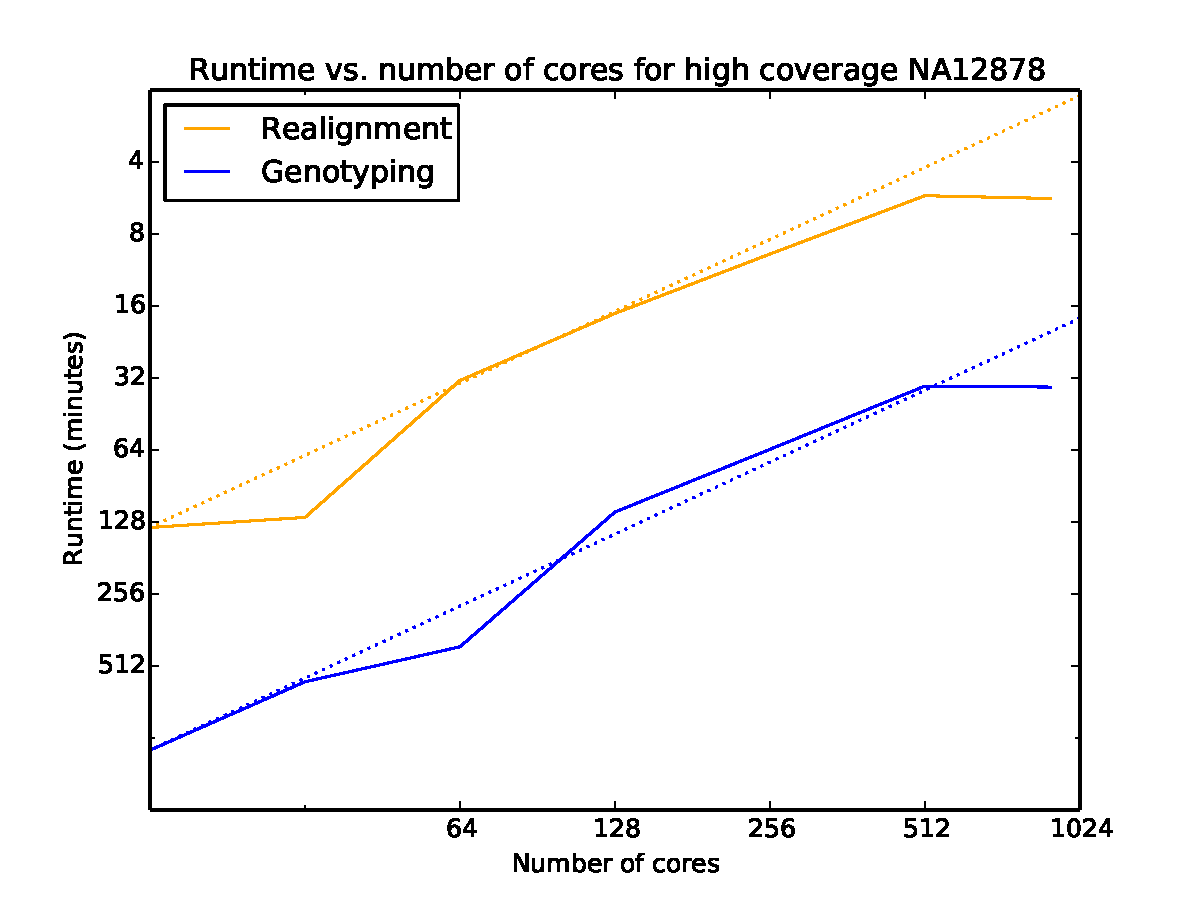
\includegraphics[width=0.95\linewidth]{graphs/speedup.pdf}
\end{center}
\caption{Runtime of the INDEL realignment and genotyping algorithms as the
number of cores is changed. Note that the times on the Y-axis are descending; as
the number of cores made available to \textsc{Avocado} is doubled, runtime
decreases. The dotted lines represent ideal scaling, where runtime halves when
the number of cores in the cluster is doubled.}
\label{fig:speedup}
\end{figure}

\textsc{Avocado} demonstrates linear strong scaling out to the full size of our
cluster. This is due to the even distribution of work across all of the nodes in
our cluster. This can be seen in Figure~\ref{fig:speedup}B, which shows that
task completion times are fairly uniform within each stage of the realignment
and genotyping process.

\begin{figure}[h]
\begin{center}
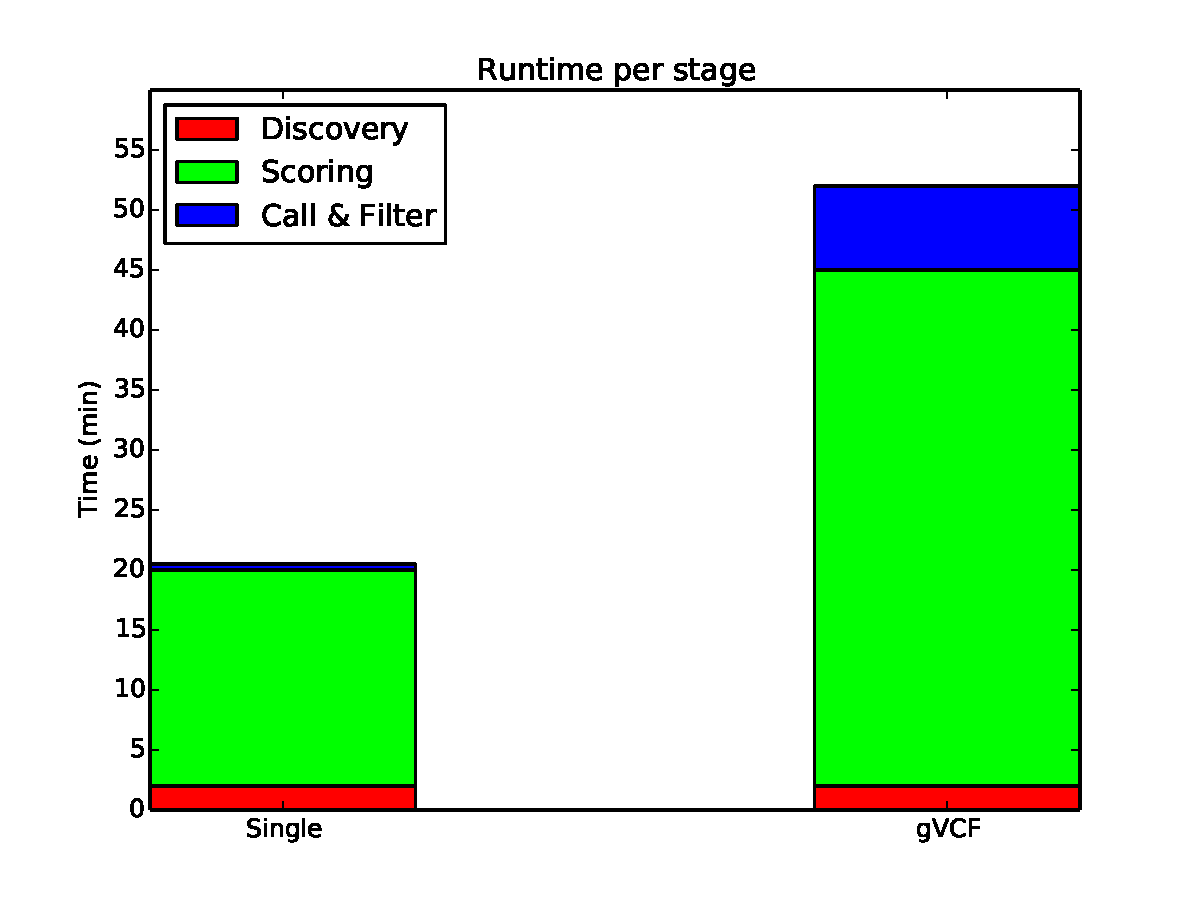
\includegraphics[width=0.95\linewidth]{graphs/perf.pdf}
\end{center}
\caption{Runtime of the different stages in the genotyper core.}
\label{fig:genotyper-perf}
\end{figure}

Figure~\ref{fig:genotyper-perf} contains a performance comparison of the
genotyping engine when running in both single sample and gVCF mode. This
comparison excludes the realignment stages, which are outside of the
genotyper core, and which are common to both stages. Loading/filtering the
input reads and discovering variants is a small fraction of the total runtime
in each mode. Scoring the variants against the reads consumes the majority of
the runtime in both modes. As we move from single sample to gVCF mode, the
time this stages takes to complete increases by $2.3\times$ from 18 minutes
to 42 minutes. This increase is expected, as we need to merge scores across
all of the sites in the genome in the gVCF mode, which drastically increases
the amount of computation we must do. This is also reflected in the final
stage, where we emit the final calls and filter variants. The runtime of this
stage increases by $14\times$ from half a minute up to seven minutes.

\section{Discussion}
\label{sec:discussion}

In addition to \textsc{Avocado}, there have been several other attempts to
develop variant callers that run using \textsc{Apache Hadoop/Spark}. An early
approach was \textsc{Crossbow}~\citep{langmead09crossbow}, which used
\textsc{Apache Hadoop} to invoke \textsc{SoapSNP}~\citep{li09snp} and
\textsc{Bowtie}~\citep{langmead09bowtie} on a cloud computing cluster.
Unlike \textsc{Crossbow}, which used \textsc{Apache Hadoop} to orchestrate
single node tools on a cluster, \textsc{Avocado} is written to natively use
\textsc{Apache Spark}'s core abstractions to run variant calling. Additionally,
there are several other variant callers under development that use
\textsc{Apache Spark}. These include
\textsc{Guacamole}\footnote{\url{https://github.com/hammerlab/guacamole/}},
which performs both germline and somatic variant calling, and the development
of the new \textsc{GATK4}\footnote{\url{https://github.com/broadinstitute/gatk}}.

Although this manuscript has focused on single sample variant calling in
\textsc{Avocado}, we also support joint variant calling across samples. When
joint calling, we support using gVCF data as input, where each site includes
likelihoods for the reference genome. We load in these likelihood observations,
and filter all sites that were called as a variant in at least one sample.
Similar to how we run genotyping~(see~\S\ref{sec:genotyping}), we overlap the
variant sites against the likelihood observations by running a join. Once we
have completed this, we use the expectation-maximization~(E-M) procedure
described in~\citet{li11} to compute the major allele frequency. We run for a
fixed number of iterations of the E-M loop before using the major allele
frequency with a binomial distribution to compensate the genotype
likelihoods. These compensated genotype likelihoods are then used to emit
a ``squared-off'' genotype matrix.

\section{Conclusion}
\label{sec:conclusion}

In this paper, we have introduced the indexed de Bruijn graph. This extension of the traditional
de Bruijn graph allows for $\Omega(n)$ local alignment of two or more sequences, with a hard
$\mathcal{O}(n)$ bound for canonical edits and an $\mathcal{O}(l^2)$ bound for non-canonical edits
(in genotyping, $l$ is the variant allele length, which is typically much smaller than $n$). After describing this structure, we have demonstrated how
indexed de Bruijn graphs can be used with a pooled model to locally reassemble haplotypes that contain
variants. By using an indexed de Bruijn graph, we are able to reduce the runtime complexity of the local
reassembly algorithms that are commonly used for variant discovery and calling.

\section*{Acknowledgements}

The authors would like to thank Timothy Danford and John St. John, who have
contributed to the architecture of Avocado through their work on somatic
variant calling, and Michael Heuer, who has been instrumental in leading
the development and refinement of \textsc{ADAM}'s variant and genotype
schemas and APIs.

\section*{Funding}

This research is supported in part by NSF CISE Expeditions Award CCF-1139158,
LBNL Award 7076018, and DARPA XData Award FA8750-12-2-0331, NIH BD2K Award
1-U54HG007990-01, NIH Cancer Cloud Pilot Award HHSN261201400006C and gifts
from Amazon Web Services, Google, SAP,  The Thomas and Stacey Siebel
Foundation, Adatao, Adobe, Apple, Inc., Blue Goji, Bosch, C3Energy, Cisco,
Cray, Cloudera, EMC, Ericsson, Facebook, Guavus, Huawei, Intel, Microsoft,
NetApp, Pivotal, Samsung, Splunk, Virdata, VMware, and Yahoo!. Author FAN is
supported by a National Science Foundation Graduate Research Fellowship.

\vspace*{-12pt}

\bibliographystyle{natbib}
%\bibliographystyle{achemnat}
%\bibliographystyle{plainnat}
%\bibliographystyle{abbrv}
%\bibliographystyle{bioinformatics}
%
%\bibliographystyle{plain}
%
\bibliography{avocado}
\end{document}
